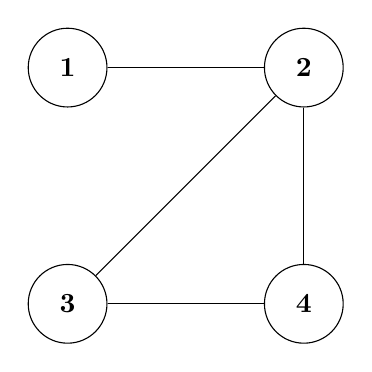
\begin{tikzpicture}[x=1.5cm, y=1.5cm]
  % 設定
  \tikzset{node/.style={circle,draw=black,minimum size=1cm}}
 
  % 補助線
  % \draw [help lines,blue] (0,0) grid (20,6);
 
  % node %
  \node[node] at (-1,1) (node1) {\textbf{1}};
  \node[node] at (1,1) (node2) {\textbf{2}};
  \node[node] at (-1,-1) (node3) {\textbf{3}};
  \node[node] at (1,-1) (node4) {\textbf{4}};
 
  \foreach \u / \v in {node1/node2, node2/node3, node2/node4, node3/node4}
  \draw (\u) -- (\v);
\end{tikzpicture}

